\chapter{Hybrid classes}\label{chap:hybrid}

\is{inflection class!hybrid}
This short chapter explores the situations where morphology allows for two different, competing strategies to be applied to the same lexeme. In inflection, this is called \isi{overabundance}, while in derivation the phenomenon is called derivational \isi{doublet}s. These systems can be modelled using hybrid classes, like the ones introduced in Chapter \ref{chap:solution}. As for the test cases, I look at Russian diminutives (derivational doublets) and Croatian instrumental singular markers (overabundance). The interesting aspect of these two cases is that there is partial overlap between class membership, which contrasts with the previous gender and inflection class cases, where a \isi{stem} or word can only belong to one inflection class at a time. In cases of affix competition and overabundance, a single lexeme can belong to two different classes at the same time, and giving speakers a choice between two formally different, but semantically identical, markers. This produces hierarchies with a different shape, which has a clear effect on the analogical relations.

\section{Overabundant inflection: Croatian singular instrumental}

\is{inflection!nominal|(}
\il{Bosnian, Croatian and Serbian|(}

In \textsc{bcs} (Bosnian, Croatian and Serbian), a number of masculine nouns belonging to the first (or \textit{-a}) declension present partial \isi{overabundance} between the markers \textit{-em} (/jem/) and \textit{-om} (/om/) in the instrumental \isi{singular}, as shown in \REF{exe-over-croat}:

\begin{exe}
    \ex \label{exe-over-croat}
    \begin{xlist}
        \ex grad-\textit{om} `city'-\textsc{instr}
        \ex muž-\textit{em} `man'-\textsc{instr}
        \ex princ-\textit{om}/princ-\textit{em} `prince'-\textsc{instr}
    \end{xlist}
\end{exe}

Importantly, not all nouns can alternate between the two markers:

\begin{exe}
    \ex \label{no-over-croat}
    \begin{xlist}
        \ex[] {kej-om `river bank'-\textsc{instr}}
        \ex[*] {kej-em}
        \ex[] {muž-em `man'-\textsc{instr}}
        \ex[*] {muž-om}
    \end{xlist}
\end{exe}


A rule of thumb for class assignment has been proposed in the literature already: ``nouns ending in a palatal \isi{phoneme} use \textit{-em}, whereas all other nouns use \textit{-om}. However, although this rule seems reasonably straightforward, there are some environments where \isi{doublet}s occur'' \autocite[377]{Lecic.2015}. Diachronically, this \isi{overabundance} \autocites{Thornton.2011, Thornton.2010a}, emerged due to the collapse of an older palatal \textit{/r$^j$/}, which justified the use of \textit{-em}, with a modern non-palatal \textit{/r/} which justifies the use of \textit{-om} \autocite{Lecic.2015}. \textcite{Mladenovic.1977} (as cited by \citealt{Lecic.2015}) claims that \textit{-om} is spreading to contexts where \textit{-em} would be historically used.

Some modern grammars give extremely general descriptions of this alternation: ``the masculine-neuter ending -om appears as -em after `soft' consonants'' \autocite[85]{Alexander.2006}.\footnote{The soft consonants in Croatian are: \textit{č, š, ž, ć, đ, dž, nj, lj, j, c}.} Similarly, other grammars seem to suggest that the alternation is purely phonological: ``Stems ending in a palatal cause vowel alternation in the instrumental singular ending, e.g. \textit{učenik\emph{o}m} `pupil' - prijateljem `friend'\dots'' \autocite[12]{Kordic.1997}. Yet other works argue that the distinction between \textit{-em} and \textit{-om} is completely predictable from whether the noun ends in a hard (\textit{-om}) or soft consonant (\textit{-em}) \autocite[146]{Hammond.2005}. Additional phonological environments of this alternation have been noted already:

\begin{quotation}
Instrumental -ет / -ем is normal with \isi{stem}s in -c, where vocative has -e/-e and the first-palatalization alternation, as ótac/отац 'father', vocative осе/оче. -от/-ом tends to be kept in foreign words and names (Kíš-от/Кйш-ом) and in words with e in the preceding syllable: padež-от/падеж-ом 'case'. \autocite[320]{Brown.1993}
\end{quotation}

\largerpage[2]
As can be seen the idea that analogical relations help predict this particular alternation is not really new. However,  \textcite{Lecic.2015} convincingly shows that for the majority of the proposed prescriptive rules of where and when to use \textit{-em} or \textit{-om}, exceptions can be found in a corpus. This essentially means that there is no obvious categorical rule that correctly predicts whether a noun will take \textit{-em}, \textit{-om} or both. Secondly, and more importantly, the author shows that overabundant nouns, even when very infrequent with one of the two forms, are acceptable for speakers, whereas non-overabundant nouns (according to the corpus) are acceptable with only one of the two forms. This strongly indicates that there really are three classes of nouns in \textsc{bcs}: \textit{-om} nouns, \textit{-em} nouns and \textit{-om/-em} nouns.
\is{exception}

\subsection{Modelling the system}

One approach how to model \isi{overabundance} with type hierarchies can be achieved by employing hybridization \autocite{GuzmanNaranjo.2016}. Hybridization assumes that there are two basic types, \textit{exclusively-em} and \textit{exclusively-om}. Nouns of type \textit{ex\-clusively-em} can only take the marker \textit{-em} and similarly for \textit{exclusively-om}. Nouns of a hybrid type \textit{em$\sim$om} can take either \textit{-em} or \textit{-om}. This hybrid type is related to the other two types as shown in \figref{fig:hybrid-bcs}.

\begin{figure}
    \caption{Hybridization in \textsc{bcs} nouns} \label{fig:hybrid-bcs} \begin{forest} baseline, %qtree edges, 
    l sep+=2em, for children={
          l sep+=2em,
        },
        for tree={
          parent anchor=south,
          child anchor=north,
          align=center,
          inner sep=1pt,
          node font=\itshape
        }
        [sg.ins
        [om, name=EM [excl-em [muž\\\emph{`man'}] [kazalište\\\emph{`theater'}]]
        [em$\sim$om, name=EMOM [princ\\\emph{`prince'}] [car\\\emph{`emperor'}]]]
        [em , name=OM [, no edge] [, no edge] [excl-om[kej\\\emph{`river bank'}] 
        [konobar\\\emph{`waiter'}]]]
        ]
        \draw (EMOM.north) -- (OM.south);
    \end{forest}
\end{figure}

In the present approach there are no \isi{constraint}s being inherited in the hierarchy in \figref{fig:hybrid-bcs}, the approach at hand simply organizes nouns according to the markers they can take in the instrumental singular. Relevant constructions or rules would then introduce the appropriate markers for each type. This can be illustrated schematically in \REF{exe-schema-new}:

\begin{exe}
    \ex \label{exe-schema-new}
    \begin{xlist}
        \ex {[}STEM(X$^{em}$)-em{]} $\leftrightarrow$ {[}SEM(X) + Inst + Sg{]}
        \ex {[}STEM(X$^{om}$)-om{]} $\leftrightarrow$ {[}SEM(X) + Inst + Sg{]}
    \end{xlist}
\end{exe}

Because lexemes like \textit{princ} and \textit{car} belong to types \textit{om} and \textit{em}, both constructions can apply to them. Other implementations are possible, of course, but the important point is that the hierarchy in \figref{fig:hybrid-bcs} expresses that nouns that can take both markers share properties with those that can take only one.

\largerpage[2]
A complex issue that arises with hybrid hierarchies is what happens to the analogical filters in such cases. The analogical function for some leaf type contains all the generalizations, as well as exceptions, that determine whether any given lexeme belongs to said type or not. In terms of the model of analogy as a type \isi{constraint}, the type \textit{em$\sim$om} inherits all analogical constraints from \textit{em} and \textit{om} as: [\textit{em$\sim$om} \textsc{phon}] = [\textit{em} \textsc{phon}] $\land$ [\textit{om} \textsc{phon}]. This means that nouns \textit{em$\sim$om} will end up looking like nouns from the classes \textit{excl-om} and \textit{excl-em}, because they must satisfy the same constraints.
\is{exception}

The prediction this approach makes is that we expect the confusion between \textit{em$\sim$om} and each of the two exclusive classes \textit{excl-em} and \textit{excl-om} to be relatively higher than the confusion between the two exclusive classes (\textit{excl-em} and \textit{excl-om}) themselves.

\subsection{Materials}

I extracted all 13227319 instances of instrumental \isi{singular} nouns from the Web Corpus of Croatian, Bosnian and Serbian \autocite{ljubesic14-bs} (1.9 billion tokens). From these, 6575746 are masculine nouns. After removing clear mistakes (punctuation marks, etc.), the total  number of types was 227263. The number of types which appeared with either \textit{-em} or \textit{-om}, or both was 186443. The final data-set (after removing cases that appeared with multiple spellings) contained 180987 nouns, with 39245 nouns (22\%) taking \textit{-em}, 137290 nouns (76\%) taking \textit{-om}, and 4452 nouns (2\%) taking both markers. Because we cannot know from a corpus whether a noun is \textit{not} over abundant, there is always the risk of have many false negatives, particularly in the lower frequency cases (since it is possible that they are overabundant but there were not enough cases in the corpus for it to appear with both markers). There is a large imbalance in the type frequency of each of the three classes. I only used \textit{-em} nouns with a frequency of more than 60, \textit{-om} nouns with a frequency of more than 500, and \textit{-em/-om} nouns with a frequency of more than 100 to address both problems. This process produces a dataset with 3138 \textit{-om} nouns, 2056 \textit{-em} nouns and 1293 \textit{-em/-om} nouns. These numbers are somewhat arbitrary, but they produce a more balanced sample and help control for false negatives. By selecting only the more frequent nouns, there is a higher probability that the class assignment is correct.

I take the \isi{stem} of the nouns to be the instrumental \isi{singular} minus the \textit{-em} or \textit{-om} endings. I performed no orthography corrections for this data-set.

\subsection{Results}

\largerpage[2]
The model is rather simple for this case. The predictors are the last two segments and the number of consonant clusters in the noun: \texttt{class $\sim$ final.1 + final.2 + n\_cluster}\footnote{This model had one hidden layer with 5 nodes and a decay rate of 0.01.}. The results of the model can be seen in \tabref{tab:ins-cro} and the corresponding statistics in \tabref{tab:ins-cro-stats}.

\begin{table}
  \centering
  \begin{tabular}{rrrrrr}
    \lsptoprule
    \multicolumn{4}{c}{Reference}                           \\
    \midrule
    Prediction & em           & em$\sim$om   & om           \\
    em         & 1887         & \emph{445} & \emph{25}  \\
    em$\sim$om & \emph{147} & 502          & \emph{188} \\
    om         & \emph{22}  & \emph{346} & 2925         \\
    \lspbottomrule
  \end{tabular}
  \caption{Confusion Matrix for the model predicting instrumental singular in Croatian nouns}\label{tab:ins-cro}
\end{table}

\begin{table}
  \centering
  \begin{tabular}{c}
    \lsptoprule
    Overall statistics:          \\
    \midrule
    Accuracy : 0.8192            \\
    95\% CI : (0.8096, 0.8285)   \\
    No Information Rate : 0.4873 \\
    Kappa : 0.7051               \\
    \lspbottomrule
  \end{tabular}
  \caption{Overall statistics for Confusion Matrix \tabref{tab:ins-cro}}\label{tab:ins-cro-stats}
\end{table}

\begin{figure}
  \centering
  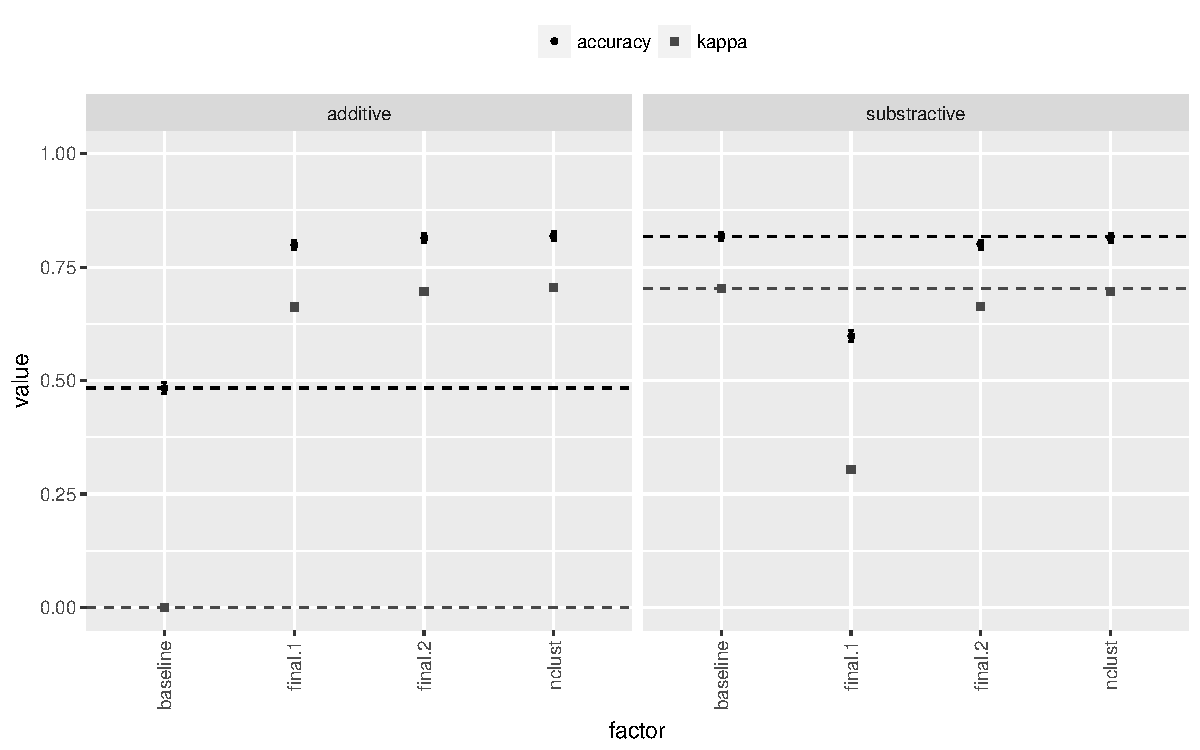
\includegraphics[width=1.0\textwidth]{./figures/croatian/factimp-plot.pdf}
    \caption{Additive (left) and subtractive (right) accuracy and kappa scores for for the model predicting Croatian instrumental}\label{fig:factimp-plot-croatian}
\end{figure}

We see that the model does predict fairly well the declension class of these nouns, although it makes a large number of mistakes when predicting \textit{-em/-om}. Most relevant here is the degree of confusion between the three classes. It can be observed that \textit{excl-om} and \textit{excl-em} have a small rate of confusion between them. The greater amount of confusion is between \textit{em}$\sim$\textit{om} and \textit{excl-em}, and \textit{em}$\sim$\textit{om} and \textit{excl-om}. This is shown more clearly in \figref{fig:croatian-results}. The Y axis shows the percentage of predicted classes for each class. We see here that  \textit{excl-em} is rarely predicted to be  \textit{excl-om} and viceversa. Meanwhile, \textit{em}$\sim$\textit{om} is often predicted to be \textit{excl-em} and \textit{excl-om}.

\begin{figure}
  \centering
  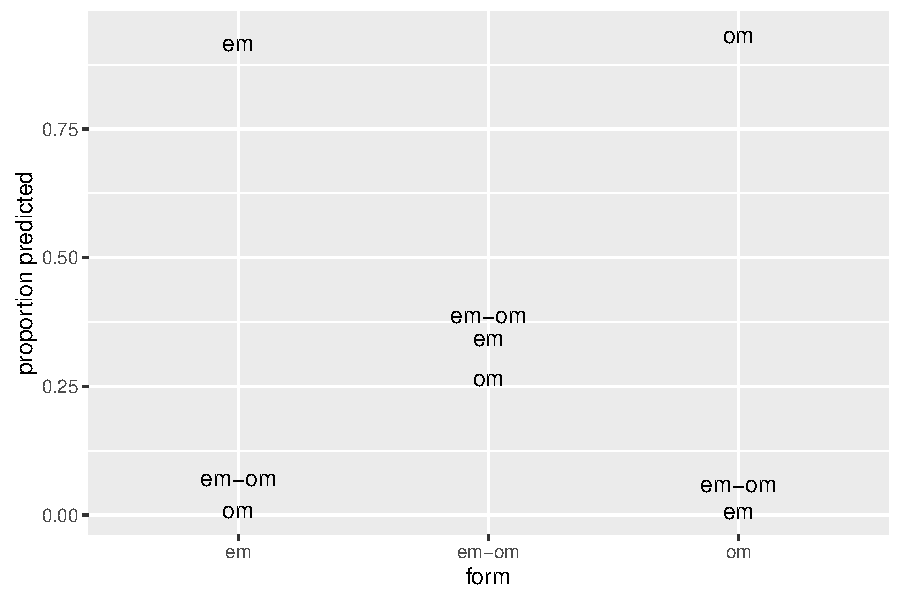
\includegraphics[width=0.8\textwidth]{./figures/croatian/croatian.pdf}
  \caption{Proportion of confusion between classes in Croatian}\label{fig:croatian-results}
\end{figure}

\largerpage[2]
This distribution is exactly what the model predicts, but it also makes sense from a historical perspective. As mentioned above, it was \textit{em} nouns which lost their distinctive \textit{r}$^j$ which started taking \textit{om}. That is, only when a certain set of \textit{em} nouns started phonological shapes which would fit the \textit{om} class, did this nouns started being overabundant. We have thus a system that went from being perfectly predictable (as already mentioned in simple cases of phonological conditioned allomorphy) to \isi{overabundance}.
\il{Bosnian, Croatian and Serbian|)}

\is{inflection!nominal|)}

\section{Frequency and analogical similarity: Russian diminutives}

\subsection{Russian diminutives}

\il{Russian|(}\is{derivation|(}%
Nouns in Russian\footnote{A previous version of the study in this section was presented in Olinco 2016 \autocite{GuzmanNaranjo.2016a}.} can form the diminutive with a wide range of different suffixes. Some examples of diminutive suffixes are shown in \REF{dims-russian}.\footnote{For clarity I will use the Latin transliterations in the examples, but the models were trained using their Cyrillic forms.}\is{diminutive}

\begin{exe}
    \ex \label{dims-russian} -jets (-ец), -ik (-ек),  -jok (-ёк), -ochik (-очек), -jechik (-ечек), -jochik (-ёчек), -itsa (-ица), -ichka (-ичка), -iko (-ико), -ko (-ко), -jetso (-ецо), -tso (-цо), -tse (-це),  \textit{-ik} (-ик),  \textit{-ok} (-ок),  \textit{-chik} (-чик)
\end{exe}

The choice of suffix is partly due to the gender of the noun \autocites{Kempe.2001, Kempe.2003}, as described in \REF{sys-dim}, but not completely. There are several possible diminutive forms for each gender, and the explanation why some nouns chose one or the other is not completely clear. As the whole system is too complex to be addressed here, I will focus on masculine nouns that build the diminutive with \textit{-ik}, \textit{-ok}, or \textit{-chik} exclusively.

\begin{exe}
    \ex \label{sys-dim}
    \begin{xlist}
        \ex -iko, -ko, -tso, -tse $\rightarrow$ neuter nouns
        \ex -itsa, -ichka $\rightarrow$ feminine nouns
        \ex -ik, -ok, -chik $\rightarrow$ masculine nouns
    \end{xlist}
\end{exe}

\largerpage
In the masculine subset: \textit{–ik}, \textit{–ok}, \textit{–chik}, we find a particularly complex affix competition problem. Example \REF{ikchikok-single} illustrates some nouns which can only appear with one of the three forms, while \REF{ikchikok-multiple} shows the nouns which occur with two of the three different markers.

\begin{exe}
    \ex \label{ikchikok-single}
    \begin{xlist}
        \ex -ik, *-chik, *-ok: stol `table', kot `cat', miač `ball'
        \ex *-ik, -chik, *-ok: zabor `fence'
        \ex *-ik, *-chik, -ok: molot `hammer', vjechjer `vening'
    \end{xlist}
\end{exe}

\begin{exe}
    \ex \label{ikchikok-multiple}
    \begin{xlist}
        \ex -ik, -chik, *-ok: stul `chair', shkaf `cabinet'
        \ex *-ik, -chik, -ok: rukav `sleeve'
        \ex -ik, *-chik, -ok: rot `mouth', list  `leaf', chas `hour'
        \ex -ik, -chik, -ok: ?
    \end{xlist}
\end{exe}

\il{German}\il{Spanish}
A similar situation can be found in German, where there is competition between the \isi{diminutive} forms \textit{-chen} and \textit{-lein}, with some degree of overlap between the two: \textit{Häuschen}$\sim$\textit{Häuslein} `small house'. Similarly, Spanish has the forms \textit{-illo}, \textit{-ito}, \textit{-cito}, \textit{-ico}, among others, and some overlap between these forms in a substantial set of nouns: \textit{casita} `small house', \textit{pollito} `chick', \textit{gatito}$\sim$\textit{gatico} `kitten'.

For Russian, there seems to be no rule-based account of which nouns can take which markers \autocite{Gouskova.2015}. Some research on Russian diminutives has focused on the relation between the different forms and gender, as well as gender acquisition \autocites{Kempe.2010, Protassova.2007, Voeykova.1998}, but relatively little attention has been given to the actual conditions that help decide between the different forms. \textcite{Gouskova.2015} is the most recent approach to this problem. The authors propose what they label sublexical phonotactics, a model that is very similar to an analogical model. The basic idea is that each form a speaker encounters is stored in a sublexicon specific to that form, i.e. \textit{-ik} forms are stored in an \textit{ik} sublexicon, \textit{-chik} forms are stored in an \textit{chik} sublexicon and so on. Speakers find phonotactic regularities in each sublexicon, and new items are coined based on those regularities. Conceptually, there are only a few minor differences between traditional analogical models and \citegen{Gouskova.2015}, but in terms of implementation some issues with the latter exist. From a theoretical perspective, \textcite{Gouskova.2015} propose a flat model, where speakers simply have lists for each type, and there is no structuring of said types. This is quite common in analogical approaches. %The real issue is that the implementation the authors propose does not actually work.

Because the issues with \citegen{Gouskova.2015} approach are of secondary concern, I will only discuss them briefly. The essence of their implementation is as follows. Using the UCLA phonotactis learner \autocite{Hayes.2008}, a first instance of their model infers phonotactic regularities in a dataset of Russian nouns marked for their \isi{diminutive} preference (the phonotactic regularities are inferred from the bases of the nouns). In a second instance, a \isi{mixed effects model} is trained on the phonotactic generalizations to determine which are statistically significant.

\largerpage[-1]
There are several problems with this method. Of some real concern is that there is no cross-validation. Their results stem from testing the model on the same dataset it was trained on; however, this could be solved. It is also somewhat unclear what the purpose of the mixed effect model is, because the UCLA learner is already predicting classes based on the phonotactic patterns. Finding statistically significant patterns is problematic because these patterns are highly correlated with each other (because of phonotactics), and mixed effects models are not robust against co-linearity, which means any statistical significance is in question.\footnote{I could not reproduce their results in order to check because the versions of the statistical software used by the authors are no longer supported.}

The results in \tabref{tab:test-gkn-model} can be obtained by looking at the predictions made by the UCLA learner\footnote{The original dataset and code used by \textcite{Gouskova.2015} were kindly provided to me by the lead author. I use the results from their code.} vs observed diminutives in the dataset. The corresponding statistics are in \tabref{tab:test-gkn-stats}. It is clear that the UCLA model is not learning to properly discriminate the diminutive classes, and the model performs at chance level.

\begin{table}
  \centering
  \begin{tabular}{lrrr}
    \lsptoprule
    & \multicolumn{3}{c}{Predicted} \\
    \midrule
    Reference & chik & ik & ok                \\
    chik      & 135  & 54 & 76                \\
    ik        & 133  & 54 & 65                \\
    ok        & 122  & 56 & 75                \\
    \lspbottomrule
  \end{tabular}
  \caption{Actual results for \citegen{Gouskova.2015} model}\label{tab:test-gkn-model}
\end{table}

\begin{table}
  \centering
  \begin{tabular}{c}
    \lsptoprule
    Overall statistics:          \\
    \midrule
    Accuracy : 0.3429\\
    95\% CI : (0.3093, 0.3776)\\
    No Information Rate : 0.5065\\
    Kappa : 0.01\\
    \lspbottomrule
  \end{tabular}
  \caption{Overall statistics for Confusion Matrix \tabref{tab:test-gkn-model}}\label{tab:test-gkn-stats}
\end{table}

In one of the tests, the authors try to evaluate their model on a wug experiment with Russian speakers. They designed 300 nonce words and asked speakers to produce the corresponding \isi{diminutive}s. The authors claim high correlation between their model and speaker choices but it is not clear how this correlation was measured. First, their evaluation is made by using Kendall's and Spearman's correlation coefficients, which would lead to believe that they are testing predicted proportions vs produced, but this is not made clear. In the code the correlation calculations are made on categorical variables, which is not advisable and makes the results hard to interpret.

Despite these potential issues, the basic idea that the affix competition in Russian diminutives is resolved analogically is on the right track. In the end, it is not of too much interest whether the phonotactics approach could outperform the neural networks I employ here, or the other way around. The important question that is left to be addressed is whether a flat list approach like that of \citegen{Gouskova.2015} is more appropriate than a structured model.

\subsection{Modelling the system}

Conceptually, if one ignores semantics and stress assignment (which also seem to have no straightforward solution according to \citealt{Gouskova.2015}), it is possible to capture the system with a cross-classification approach similar to the Croatian system.

The hierarchy in \figref{fig:hierarchy-russ} shows an simple sketch of how the system can be captured. \figref{fig:hierarchy-russ} shows that all pairwise combinations are possible.\footnote{I am not aware of cases where all three suffixes are possible with one noun and could not elicit any from my informants.}

\begin{figure}
    \caption{Hybridization in Russian nouns} \label{fig:hierarchy-russ}
    \begin{forest} baseline, qtree, node font=\itshape, 
    l sep+=2em, for children={
          l sep+=2em,
        }
        [DIM
        [\dots]
        [,no edge]
        [,no edge]
        [\textit{IK}, name=IK [\textit{ik}] [{\textit{ik$\sim$chik}}, name=IKCHIK]]
        [\textit{CHIK} , name=CHIK [\textit{chik}] [\textcolor{gray}{\textit{ik$\sim$chik$\sim$ok}}, edge=densely dotted, name=IKCHIKOK]]
        [\textit{OK}, name=OK [\textit{ok}] [\textit{ik$\sim$ok}, name=IKOK] [\textit{chik$\sim$ok}, name=CHIKOK]]
        [,no edge]
        [,no edge]
        [\dots]]
        \draw (IKOK.north) -- (IK.south);
        \draw (IKCHIK.north) -- (CHIK.south);
        \draw (CHIKOK.north) -- (CHIK.south);
        \draw[densely dotted] (IKCHIKOK.north) -- (IK.south);
        \draw[densely dotted] (IKCHIKOK.north) -- (OK.south);
    \end{forest}
\end{figure}

Since all combinations are possible, we expect confusion between all three types. However, the frequency at which the combinations occur is not uniform. \figref{fig:freqs-russ-dims} shows that the most frequent classes are the non alternating classes and the \textit{ik$\sim$ok} class (see the next section for details on the dataset used). This case is thus interesting because it shows the effects of type frequency. If type frequency plays no role, then we would expect that the confusion between \textit{ik}, \textit{ok} and \textit{chik} should be more or less equal. If, on the other hand, type frequency does play a role, we expect confusion between all classes, with the highest confusion between \textit{ik}, \textit{ok} and \textit{ik$\sim$ok}, while the lowest confusion should be between \textit{chik} and \textit{ik$\sim$ok} (since this combination was not attested).

\begin{figure}
  \centering
  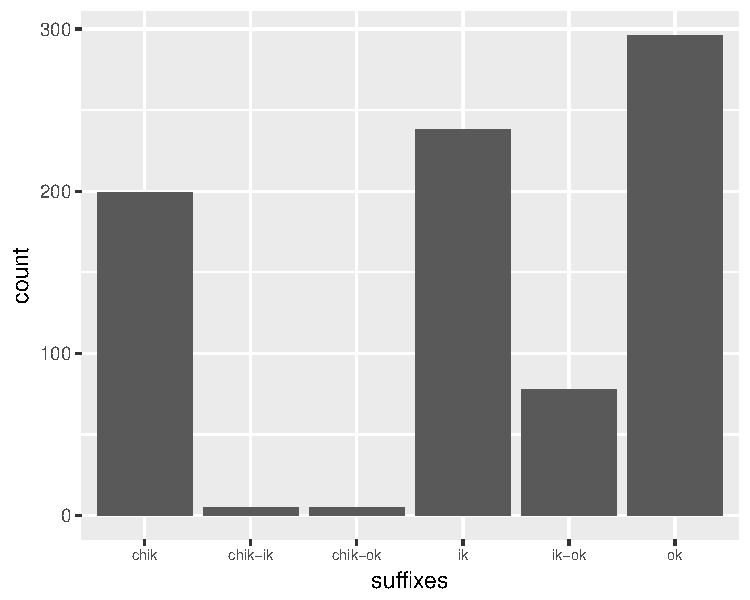
\includegraphics[scale=0.7]{./figures/russian/suffixes}
  \caption{Type frequency of Russian suffix classes}\label{fig:freqs-russ-dims}
\end{figure}

\subsection{The dataset}
\largerpage
I used the diminutive dataset collected by \textcite{Gouskova.2015}, but hand checked them with a native speaker of Russian.\footnote{This part of the work would not have been possible without the invaluable help of Elena Pyatigorskaya, who manually checked and corrected the whole-data set.} The original dataset was extracted from the google-ngram corpus \autocite{Michel.2011} and contains 1367 forms. Since there are no Russian taggers which can identify diminutives, the authors relied exclusively on the endings of the words to find diminutive forms. This caused the dataset to have many problematic cases. To solve this, we removed errors (perceived to be ungrammatical by a few informants), non-diminutives (e.g. the word \textit{alkogol-ik} `alcoholic' has an \textit{-ik} suffix but is not actually a diminutive) and non-words. This left us with 821 diminutives. My informant provided stress marks for the bases of the selected diminutives.

Because there are not enough cases for the classes \textit{chik$\sim$ok} (f=7) and \textit{chik$\sim$ik} (f=8), I removed them from the data set for fitting the models.\footnote{These two classes were not predictable at all if included. It is hard to tell whether a model with more examples would perform better in these two cases.} The final dataset had a total of 811 nouns.

\subsection{Results}

\largerpage
To predict the diminutive forms, I fitted a model using the formula: \texttt{diminutive $\sim$
  final.1 + final.2 + length\_letters * n\_vowels + stress\_position * stressed\_vowel}. Basically, this model looks at the final two segments of the base nouns (in the nominative), the interaction between the length of the base and the number of vowels of the base, the position of the stress in the word (counting from the right) and the stressed vowel. The results can be seen in \tabref{tab:dim-russ} and the corresponding statistics in \tabref{tab:dim-russ-stats}. The relative importance of the predictors is shown in \figref{fig:factimp-plot-russian}.

\begin{table}
  \centering
  \begin{tabular}{rrrrr}
    \lsptoprule
    \multicolumn{5}{c}{Reference}               \\
    \midrule
    Prediction  & chik & ik  & ik$\sim$ok & ok  \\
     chik       & 177  & 11  & 1          & 13  \\
     ik         & 8    & 175 & 28         & 33  \\
     ik$\sim$ok & 1    & 22  & 34         & 18  \\
     ok         & 13   & 30  & 15         & 232 \\
    \lspbottomrule
  \end{tabular}
  \caption{Confusion Matrix for the model predicting Russian diminutives}\label{tab:dim-russ}
\end{table}

\begin{table}
  \centering
  \begin{tabular}{llrrr}
    \lsptoprule
    \multicolumn{5}{c}{Overall statistics:} \\

    \midrule
    \multicolumn{5}{c}{Accuracy : 0.762}\\
    \multicolumn{5}{c}{95\% CI : (0.7312, 0.791)}\\
    \multicolumn{5}{c}{No Information Rate : 0.365}\\
    \multicolumn{5}{c}{Kappa : 0.6654}\\
    \lspbottomrule
  \end{tabular}
  \caption{Overall statistics for Confusion Matrix \tabref{tab:dim-russ}}\label{tab:dim-russ-stats}
\end{table}

\begin{figure}
  \centering
  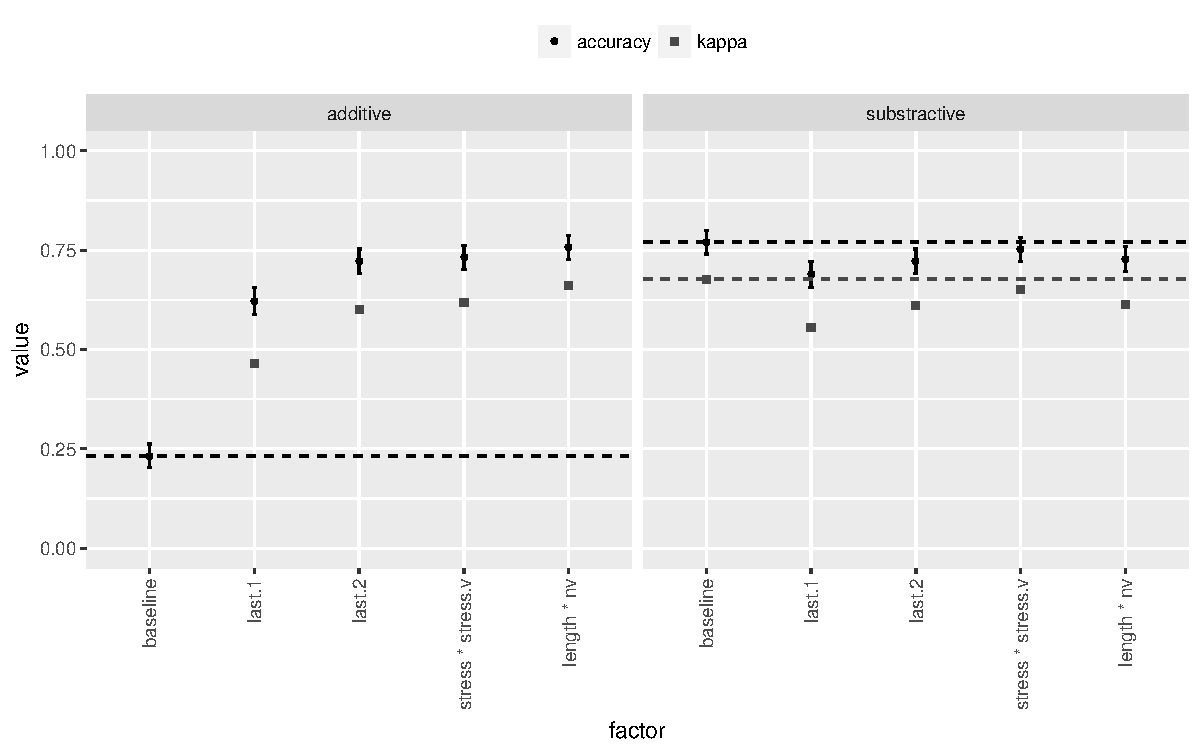
\includegraphics[width=1.0\textwidth]{./figures/russian/factimp-plot.pdf}
    \caption{Additive (left) and sbustractive (right) accuracy and kappa scores for the model predicting Russian diminutives}\label{fig:factimp-plot-russian}
\end{figure}

First of all, the model is very accurate overall and well above random chance. All four classes can be distinguished to a certain degree. The most important factor is the last segment, but the other factors all seem to have an important effect. More importantly, we find the exact predicted result in the error distribution. The class \textit{ik$\sim$ok} is less confused with the class \textit{chik} than with any of the other classes. Class \textit{chik} is rarely confused with classes \textit{ik} and \textit{ok}, while these two are confused with each other with relatively high frequency. This is clearly shown in \figref{fig:russian-results}.

\begin{figure}
  \centering
  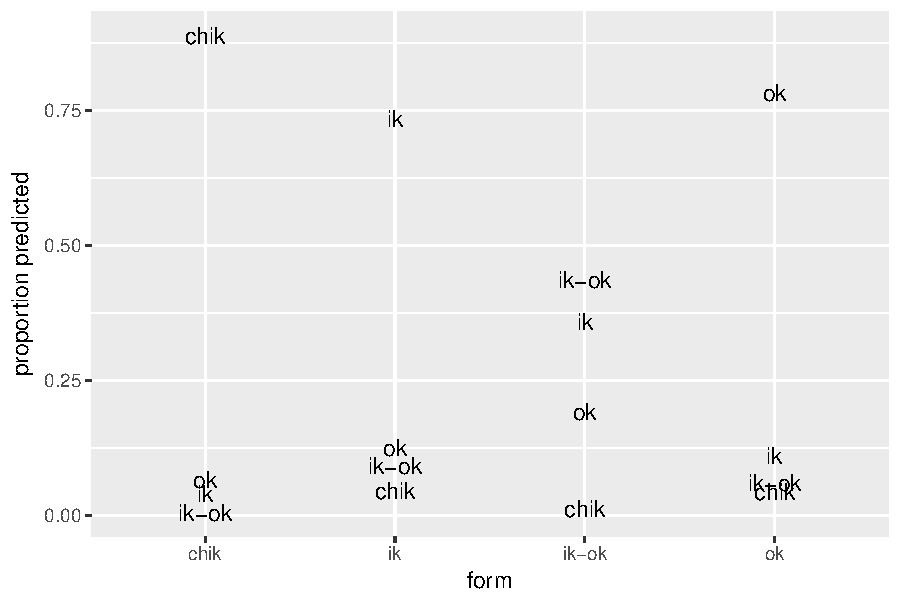
\includegraphics[width=0.8\textwidth]{./figures/russian/rus.pdf}
  \caption{Proportion of confusion between classes in Russian}\label{fig:russian-results}
\end{figure}


There are two ways how to interpret these findings. Firstly, in one scenario, it could be postulated that there is a need for quantitative information to be hard coded into the hierarchy, i.e. we should assign stronger connections to \textit{IK} and \textit{OK}, than to the other combinations. I propose, however, that this addresses the problem backwards. The more straightforward alternative is to see the higher type frequency of \textit{ik$\sim$ok} as a byproduct of the analogical system itself, and not as something one has to directly integrate into the model. The fact that we have more \textit{ik$\sim$ok} nouns than \textit{chik$\sim$ik} or \textit{chik$\sim$ok} nouns is due to the \isi{constraint}s for \textit{IK} and \textit{OK} being more compatible with each other, and producing a more relaxed set of constraints than \textit{CHIK$\sim$IK} or \textit{CHIK$\sim$OK}.

\il{Russian|)}
\is{derivation|)}

\section{Interim conclusion}

I have shown how the hybridization model can properly predict the distribution of both partially overlapping cases in Croatian, and overlapping diminutives with different type frequencies in Russian. These two examples show that the predicted effects are not only present in simple trees, but can be also observed in more complex hierarchical structures. These results clearly reject the flat list approach and support a structured organization of these systems. It is also interesting to see that, despite the fact that one case is inflectional morphology and the other derivational morphology, the results for both studies are very similar in terms of the distribution of errors and the analogical relations. This result argues for an organization of the \isi{stem}s in classes independent of the type of morphological process, at least for morphological theories that make a distinction between inflection and derivation. So, even if \isi{overabundance} in inflection and affix competition in derivation are treated as different kind of phenomena, the underlying structures would be equivalent.

%%% Local Variables:
%%% mode: latex
%%% TeX-master: "../main"
%%% End:
